\documentclass[sigconf, review, anonymous, capitalise]{acmart}
% capitalise option is for cleveref

\usepackage{tcolorbox}
\usepackage{listings}
\usepackage{tikz}
% \usepackage{flafter}
\usepackage{booktabs}
\usepackage{subfig}

\usetikzlibrary{calc}
\usetikzlibrary{graphs}
\usetikzlibrary{shapes}
\usetikzlibrary{positioning}
\usetikzlibrary{arrows.meta}

\lstloadlanguages{PHP}
\lstset{language=PHP,basicstyle=\small\ttfamily}


% Copyright
%\setcopyright{none}
%\setcopyright{acmcopyright}
%\setcopyright{acmlicensed}
\setcopyright{rightsretained}
%\setcopyright{usgov}
%\setcopyright{usgovmixed}
%\setcopyright{cagov}
%\setcopyright{cagovmixed}


% DOI
\acmDOI{}

% ISBN
\acmISBN{}

%Conference
\acmConference[Koli Calling '17]{17th Koli Calling International Conference on Computing Education Research}{November 2017}{Koli, Finland} 
\acmYear{2017}
\copyrightyear{2017}

\acmPrice{}


\title{Semi-automated grading of SQL \\ schemas using database unit testing}
\author{Nigel Stanger}
\orcid{orcid.org/0000-0003-3450-7443}
\affiliation{
    \institution{University of Otago}
    \department{Department of Information Science}
    \city{Dunedin}
    \country{New Zealand}
}
\email{nigel.stanger@otago.ac.nz}

\begin{document}

\begin{abstract}
    A key skill that students must learn when studying relational database concepts is how to design and implement a database schema in SQL. This skill is often tested using an assignment where students derive an SQL schema from a natural language specification. Grading of such assignments can be complex and time-consuming, and novice database students often lack the skills to evaluate whether their implementation accurately reflects the specification's requirements. In this paper we describe a novel semi-automated system for grading student-created SQL schemas, based on a unit testing model. The system verifies whether the schema conforms to a machine-readable version of the specification, and runs in two modes: a staff mode for grading, and a reduced functionality student mode that students can use to check whether their schema meets minimum requirements. Analysis of student performance over the period this system was in use shows evidence of improved grades as a result of students using the system.
\end{abstract}

\begin{CCSXML}
<ccs2012>
<concept>
<concept_id>10003456.10003457.10003527.10003540</concept_id>
<concept_desc>Social and professional topics~Student assessment</concept_desc>
<concept_significance>500</concept_significance>
</concept>
<concept>
<concept_id>10002951.10002952.10003197.10010822.10010823</concept_id>
<concept_desc>Information systems~Structured Query Language</concept_desc>
<concept_significance>300</concept_significance>
</concept>
<concept>
<concept_id>10002951.10002952.10003190.10003206</concept_id>
<concept_desc>Information systems~Integrity checking</concept_desc>
<concept_significance>100</concept_significance>
</concept>
<concept>
<concept_id>10010405.10010489.10010490</concept_id>
<concept_desc>Applied computing~Computer-assisted instruction</concept_desc>
<concept_significance>300</concept_significance>
</concept>
<concept>
<concept_id>10011007.10011074.10011099.10011102.10011103</concept_id>
<concept_desc>Software and its engineering~Software testing and debugging</concept_desc>
<concept_significance>100</concept_significance>
</concept>
</ccs2012>
\end{CCSXML}

\ccsdesc[500]{Social and professional topics~Student assessment}
\ccsdesc[300]{Information systems~Structured Query Language}
\ccsdesc[100]{Information systems~Integrity checking}
\ccsdesc[300]{Applied computing~Computer-assisted instruction}
\ccsdesc[100]{Software and its engineering~Software testing and debugging}

\keywords{automated grading, SQL, database schema, data definition language (DDL), student performance, unit testing}

\maketitle


\section{Introduction}

Any introductory database course needs to cover several core concepts, such as what is a database, what is a logical data model, and how to create and interact with a database. Typically such courses focus on the relational model and its embodiment in SQL database management systems (DBMSs). This is because the relational model provides a sound theoretical framework for discussing key database concepts \cite{Date.C-2009a-SQL-and-Relational}, and because SQL DBMSs are so widely used. The shadow of SQL is so strong that even non-relational systems have adopted some form of SQL-like language in order to leverage existing knowledge (e.g., OQL \cite{Cattell.R-2000a-ODMG3}, HiveQL \cite{Apache-2017a-Hive}, and CQL \cite{Apache-2017a-CQL}).

Courses that teach SQL usually include one or more assessments that test students' ability to create a database using SQL data definition (DDL) statements, and to interact with the database using SQL data manipulation (DML) statements. Manually grading the code submitted for such assessments can be a slow, tedious, and potentially error-prone process. Automated or semi-automated grading has been shown to improve turnaround time and consistency, and is generally received positively by students \cite{Douce.C-2005a-Automatic,Russell.G-2004a-Improving,Dekeyser.S-2007a-Computer,Prior.J-2004a-Backwash}. If the grading can be done in real time, the grading tool can even become part of a larger, interactive SQL learning environment (e.g.,  \cite{Kenny.C-2005a-Automated,Kleiner.C-2013a-Automated,Mitrovic.A-1998a-Learning,Russell.G-2004a-Improving,Sadiq.S-2004a-SQLator}).

While there have been many prior efforts to automatically or semi-automatically grade SQL DML (see \cref{sec-literature}), there appear to have been no corresponding efforts to grade SQL \emph{DDL}. There are generally two main aspects that need to be considered when grading an SQL schema implementation. First, is the DDL code (i.e., \texttt{CREATE} statements) syntactically correct? This is already dealt with quite effectively by the syntax checkers built into every SQL DBMS (although it is fair to say that the errors produced by such checkers can sometimes be obscure and unhelpful). A student who submits code containing syntax errors cannot expect to score well! A related aspect is code style (e.g., naming, formatting, indentation), but we do not consider this here.
    
Second, does the schema meet the requirements of the problem being solved? A database schema is normally designed and implemented within the context of a specific set of requirements, so verifying that the implemented SQL schema fulfills these requirements is an effective way to grade the implementation, and also provides a useful framework for providing feedback to students. The requirements for a database schema can be loosely divided into \emph{structure} (e.g., tables, columns, data types), \emph{integrity} (e.g., keys, constraints), and \emph{behavior} (e.g., sequences, triggers).

In this paper we describe a novel system that semi-automates the grading of students' SQL schema implementations. The system takes as input a machine-readable specification of the assessment requirements and a live instance of a submitted student schema, and verifies whether the schema conforms to the specification. Rather than attempt to parse and check the \texttt{CREATE} statements directly, the system verifies the structure of the schema by issuing queries against the schema's metadata (catalog) to look for expected values such as table names, column names, etc. It verifies integrity constraints by attempting to insert known legal and illegal values. The system currently does not check behavioral aspects. The results of the tests are compared against the machine-readable specification. This process is effectively one of unit testing the schema using the specification as a framework. We use the PHPUnit database unit testing framework to carry out this process, albeit in a somewhat unorthodox way (see \cref{sec-design}).

The remainder of the paper is structured as follows. In the next section we discuss related work, while \cref{sec-motivation} discusses the motivation and context for our approach. \Cref{sec-design} discusses the design of our system, and \cref{sec-evaluation} evaluates its impact. We discuss known issues and future work in \cref{sec-issues}, and conclude in \cref{sec-conclusion}.


\section{Related work}
\label{sec-literature}

There have been many prior efforts to build systems to support students who are learning SQL. Early examples such as RDBI \cite{Dietrich.S-1993a-An-educational} and esql \cite{Kearns.R-1997a-A-teaching} were essentially just query execution environments that students could use to practice writing SQL queries. RDBI provided relatively little feedback about the correctness of a query, whereas esql could visualize the intermediate tables generated by each step of a query, enabling students to better understand the steps in its execution.

Later systems became more responsive in terms of the feedback they provided to students. Systems like SQL-Tutor \cite{Mitrovic.A-1998a-Learning}, SQLator \cite{Sadiq.S-2004a-SQLator}, AsseSQL \cite{Prior.J-2004a-Backwash}, ActiveSQL\footnote{\url{https://db.grussell.org/}} \cite{Russell.G-2004a-Improving,Russell.G-2005a-Online}, SQLify \cite{Dekeyser.S-2007a-Computer}, and aSQLg \cite{Kleiner.C-2013a-Automated} all provided varying levels of syntactic and semantic feedback. Many of these took a more ``functional'' approach to checking SQL query code, i.e., verifying that the code written fulfilled the requirements of the problem, rather than focusing on the code itself. This was most commonly done by checking how much the result set of a student's query differed from the correct result set (e.g., SQLator's ``equivalence engine'' \cite{Sadiq.S-2004a-SQLator}). ActiveSQL could also detect ``hard-coded'' queries that produced the desired result, but which would fail if the data set changed \cite{Russell.G-2005a-Online}. The SQL Exploratorium \cite{Brusilovsky.P-2010a-Learning} took an interesting alternative approach, using parameterized query templates to generate the questions given to students.

Given the relatively static nature of an SQL schema, we feel this verification style of approach is the most appropriate way of constructing an automated grading system for SQL DDL. As an aside, the concept of verifying a schema against its specification sounds like it should be a useful application of formal methods \cite{Spivey.J-1989a-An-introduction}, but work with formal methods and databases has historically focused either on \emph{generating} a valid schema from a specification (e.g., \cite{Vatanawood.W-2004a-Formal,Lukovic.I-2003a-Proceedings,Choppella.V-2006a-Constructing}), or on verifying schema transformation and evolution \cite{Bench-Capon.T-1998a-Report}. A formal methods approach could certainly be used to generate the model answer or rubric for grading an assessment, but this is effectively the inverse of what is needed to grade a student-written schema.

Previous systems focused almost exclusively on SQL \emph{queries} using the \texttt{SELECT} statement (i.e., DML) rather than SQL \emph{schema definitions} (DDL). This focus is unsurprising given that \texttt{SELECT} is probably the most frequently used of any SQL statement, and also because it is relatively complex compared to most other SQL statements. Only a few of systems we reviewed even mentioned schema definition. RDBI \cite{Dietrich.S-1993a-An-educational} supported a DDL, but only its own non-SQL language, while esql \cite{Kearns.R-1997a-A-teaching} simply passed anything that was not a \texttt{SELECT} statement through to the DBMS. \citeauthor{Gong.A-2015a-CS-121-Automation}'s ``CS 121 Automation Tool'' \cite{Gong.A-2015a-CS-121-Automation} focuses primarily on SQL DML statements, but appears to be extensible and could potentially be modified to support SQL DDL statements.

Many previous systems have implemented some form of automated or semi-automated grading, e.g., SQLator \cite{Sadiq.S-2004a-SQLator}, AssesSQL \cite{Prior.J-2004a-Backwash}, ActiveSQL \cite{Russell.G-2004a-Improving,Russell.G-2005a-Online}, SQLify \cite{Dekeyser.S-2007a-Computer}, aSQLg \cite{Kleiner.C-2013a-Automated}, \citeauthor{Gong.A-2015a-CS-121-Automation}'s ``CS 121 Automation Tool'' \cite{Gong.A-2015a-CS-121-Automation}, and XDa-TA\footnote{\url{http://www.cse.iitb.ac.in/infolab/xdata/}} \cite{Bhangdiya.A-2015a-XDa-TA,Chandra.B-2015a-Data,Chandra.B-2016a-Partial}. Some (e.g., SQLator, AssesSQL) provided only correct/incorrect responses, while others (e.g, ActiveSQL, SQLify, aSQLg, XDa-TA) had more sophisticated schemes for assigning partial credit, such as ActiveSQL's accuracy score, SQLify's eight-level scale, and XDa-TA's ability to generate data sets designed to catch common errors. In either case, these systems were often able to automatically mark a significant fraction (e.g., about a third for SQLator \cite{Sadiq.S-2004a-SQLator}) of submitted queries as correct without human intervention, thus reducing marking load for teachers.

To our knowledge there has been no work on automated grading of SQL DDL statements. While dealing with \texttt{CREATE} statements should be simpler than dealing with \texttt{SELECT} statements, the ability to at least semi-automate the grading of SQL schema definitions should reap rewards in terms of more consistent application of grading criteria, and faster turnaround time \cite{Douce.C-2005a-Automatic,Russell.G-2004a-Improving,Dekeyser.S-2007a-Computer,Prior.J-2004a-Backwash}.

Another branch of related work is systems that actively aid students in learning SQL, e.g., SQL-Tutor \cite{Mitrovic.A-1998a-Learning}, SQLator \cite{Sadiq.S-2004a-SQLator}, ActiveSQL \cite{Russell.G-2004a-Improving}, and aSQLg \cite{Kleiner.C-2013a-Automated}. SQL-Tutor is a typical example of this category. It was an intelligent teaching system that provided students with a guided discovery learning environment for SQL queries, and used constraint-based modeling \cite{Ohlsson.S-1992a-Constraint-based,Ohlsson.S-2016a-Constraint-based} to provide feedback to students. \citeauthor{Kenny.C-2005a-Automated} \cite{Kenny.C-2005a-Automated} described a similar SQL learning system that incorporated an assessment of a student's previous progress. This enabled a more personalized and adaptive approach to student learning, where feedback was tailored according to student progress.

There is relatively little prior work on unit testing of databases. Most authors working in this area have focused on testing database \emph{applications} rather than the database itself (e.g., \cite{Binnig.C-2008a-Multi-RQP,Chays.D-2008a-Query-based,Marcozzi.M-2012a-Test,Haller.K-2010a-Test}). \citeauthor{Ambler.S-2006a-Database} discusses how to test the functionality of a database \cite{Ambler.S-2006a-Database}, while \citeauthor{Farre.C-2008a-SVTe} describe how to test the ``correctness'' of a schema \cite{Farre.C-2008a-SVTe}, focusing mainly on consistency of constraints. Neither consider how to verify that a database schema conforms to the requirements of the original specification.


\section{Motivation}
\label{sec-motivation}

Since 1989, our department has offered some form of mandatory database concepts course, typically one semester during the second year\footnote{New Zealand Bachelor's degrees normally comprise three years of study.} of study, building on a short introduction to basic data management concepts in the first year. Typical of courses of this nature, it covered core topics such as the relational model, relational algebra, data integrity, SQL DDL and DML, and a varying mixture of other database topics such as transactions, concurrency control, triggers, and security. Assessment of SQL skills was typically carried out using a mixture of assignments and tests.

From 2001 to 2003, we assessed students' SQL DDL skills with an in-lab practical examination. Students were given a fictional scenario specification, and had 100 minutes in which to modify a provided schema template with additional tables, constraints, etc. The test was generally easier to grade than the more ``realistic'' practical assignment that we had used in earlier years, as the scenario specification tended to be quite tightly specified and thus less open to (mis)interpretation. However, the test experience was quite stressful to students due to the limited timeframe and limited access to online references. We did not attempt to automate the grading of these tests.

The most common approach we have used to assess students' SQL DDL skills was a practical assignment, where students had 3--4 weeks in which to implement a database schema based on a fictional scenario specification. The scenario posed that the student was a database developer involved in a larger project, and that the specification was the output of the requirements analysis phase. An entity-relationship diagram (ERD) of a typical scenario that we used (known as the ``BDL'' scenario) is shown in \cref{fig-ERD}.
 
 
\begin{figure}[hb]
    \centering
    \includegraphics[width=0.85\columnwidth, keepaspectratio]{images/BDL_ERD.pdf} 
    \caption{ERD of the ``BDL'' scenario used to assess SQL DDL skills (Information Engineering notation).}
    \label{fig-ERD}
\end{figure}


Prior to 2001, the specifications for the scenarios used in this assignment were deliberately somewhat loosely defined and often contained areas that were under-specified or ambiguous. At the time the course also included some data modeling content, so this approach enabled students to explore the different ways that a conceptual model could be converted into an implementation. This of course led to variation across student submissions, due to differing interpretations of the under-specified elements. Automation of grading was problematic, especially when students chose different database structures, or different names for tables and columns, than what was ``expected''. We therefore made no significant attempt to automate grading under this approach.

By 2004 the data modeling content was being migrated into other courses, so we took the opportunity to tighten up the scenario specifications to reduce ambiguity. In 2013 we took the further step of ``freezing'' the specification, i.e., students were not permitted to make arbitrary changes to the specification without strong justification, and even then only if the changes did not impact how client programs interacted with the database. For example, if a column needed to be restricted to a discrete set of values, a student could---if they wished---choose to go beyond the specification and enforce this requirement using a separate lookup table rather than a \texttt{CHECK} constraint, as long as this did not change the originally specified structure of the table. This meant that students could still exercise some flexibility in their schema implementations where appropriate, and ensured that the assignment was not just a mechanical translation exercise.

The in-scenario rationale for freezing the specification was that other developers were independently using the same specification to code end-user applications. Any significant variation from the specification would therefore break those applications. This approach tested not only students' ability to write SQL DDL, but also their ability to correctly interpret and convert a natural language database specification into a corresponding SQL schema.

This approach seemed effective, but maintaining consistent grading standards across a large number of submissions (on the order of 50--70) was difficult, due the often large number of distinct gradable elements implied by the specification. This required a complex and highly-detailed rubric to be constructed so that no element was missed, and the grading process consequently took a significant amount of time, especially when feedback to students was required. In 2012 a significant change to the structure of the course resulted in higher grading workloads and increased time pressure, prompting greater interest in the possibility of at least semi-automating the grading of this assignment. This was now more feasible than in earlier years due to the more tightly constrained nature of the project specification.

Another motivation for automated grading was that it can sometimes be difficult for database novices to know whether they are on the right track while implementing a specification. If a limited version of the grading tool was available to students before the submission deadline, it could be used to provide feedback on their progress.

We decided to define a minimum set of requirements for the assignment: students' SQL code should be syntactically correct, and it should include all tables and columns---with correct names and appropriate data types---as detailed in the specification. If a student satisfied these minimum requirements, they were guaranteed to score at least 50\%. They could check whether their schema met these requirements prior to the deadline by submitting their schema for checking through a web application. That way they (and we) could be more certain that at least the core structure of their schema was correct. After the deadline, teaching staff used a console application to check for correct implementation of other aspects of the schema, such as integrity constraints.

We trialled a prototype of the staff-facing application in 2012, and rolled out the student-facing application in 2013.


\section{System design}
\label{sec-design}

The architecture of our system is shown in \cref{fig-architecture}. Its core function is to check whether a student's schema conforms to the assignment specification, by automatically comparing their schema submission against a machine-readable version of the specification. This is essentially a unit testing approach, so we decided to build the system around an existing unit testing framework.


\begin{figure}[h]
    \sffamily
    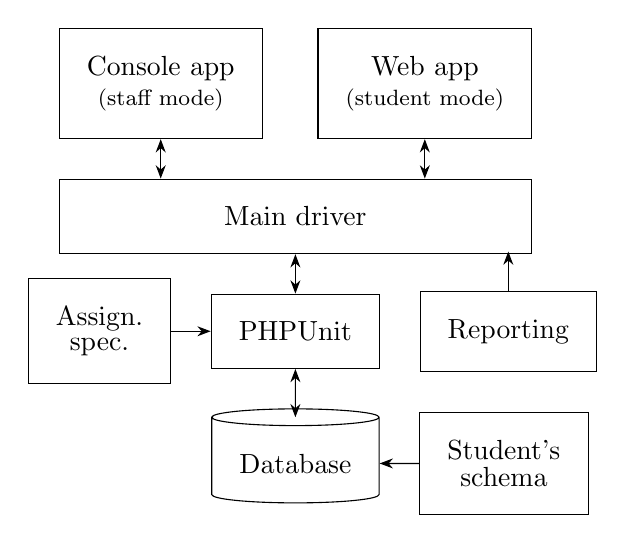
\begin{tikzpicture}[every node/.style={draw, minimum height=7.5mm, inner sep=1em}]
        \node (console) {\shortstack{Console app \\ \footnotesize(staff mode)}};
        \coordinate[below=5mm of console.south] (console port);
        
        \node[anchor=north west, minimum width=6cm] (driver) at ($(console.south west) - (0,5mm)$) {Main driver};
        
        \node[anchor=south east] (web) at ($(driver.north east) + (0,5mm)$) {\shortstack{Web app \\ \footnotesize(student mode)}};
        \coordinate[below=5mm of web.south] (web port);
        
        \node[below=5mm of driver] (phpunit) {PHPUnit};
        
        \node[left=5mm of phpunit] (spec) {\shortstack{Assign. \\ spec.}};
        
        \node[right=5mm of phpunit] (reporting) {Reporting};
        \coordinate[above=5mm of reporting.north] (reporting port);
        
        \node[cylinder, shape border rotate=90, below=5mm of phpunit, aspect=0.1] (database) {Database};
        
        \path (database.before top) -- (database.after top) coordinate[midway] (dbtop);
        
        \node[right=5mm of database] (schema) {\shortstack{Student's \\ schema}};
        
        \graph { [edges={draw, arrows={{Stealth}-{Stealth}}}]
            {(console), (web)} -> {(console port), (web port)},
            (driver) -> (phpunit),
            (phpunit) -> (dbtop),
        };
        
        \graph { [edges={draw, arrows={-{Stealth}}}]
            (reporting) -> (reporting port),
            (spec) -> (phpunit),
            (schema) -> (database),
        };
    \end{tikzpicture}
    \caption{System architecture.}
    \label{fig-architecture}
\end{figure}


There are surprisingly few frameworks for performing unit tests that interact with a database, probably due to the complexities involved. In conventional application unit testing it is relatively simple to create mocked interfaces for testing purposes. With a database, however, we need to create tables, populate them with appropriate test data, verify the state of the database after each test has run, and clean up the database for each new test \cite{Bergmann.S-2017a-PHPUnit}. Cleaning up is particularly crucial, as the order of tests is often not deterministic, i.e., the tests are not guaranteed to run in exactly the same order each time. Tests that change the state of the database may therefore affect the results of later tests in unpredictable ways.

We are aware of only four unit testing frameworks that provide specific support for database unit tests: DbUnit for Java,\footnote{http://dbunit.sourceforge.net/} DbUnit.NET,\footnote{http://dbunit-net.sourceforge.net/} Test::DBUnit for Perl,\footnote{http://search.cpan.org/~adrianwit/Test-DBUnit-0.20/lib/Test/DBUnit.pm} and PHPUnit.\footnote{https://phpunit.de/} We chose to implement the system in PHP, as it enabled us to quickly prototype the system and simplified development of the student-facing web application. A similar approach could be taken with any of the other frameworks, however.

Our database teaching was mainly based around Oracle, but the system could be adapted relatively easily for use with any DBMS supported by PHP's PDO extension. This would require implementing an additional layer to abstract the internal details of how each DBMS structures its catalog tables.

The core of the system is the \textsf{Main driver} component (see \cref{fig-architecture}). This can execute in either \emph{student mode}, which runs only a subset of the available tests, or in \emph{staff mode}, which runs all available tests (the nature of these tests will be discussed in more detail shortly). The mode is determined by the client application, as shown in \cref{fig-architecture}. Currently student mode is accessed through a web application, while staff mode is accessed through a console application, but each could easily be implemented in a variety of different ways. The main driver uses the \textsf{Reporting} module to generate test output in either HTML or plain text, as appropriate.

The assignment specification (\textsf{Assign.\ spec.} in \cref{fig-architecture}) is encoded as a collection of subclasses of PHPUnit's \texttt{TestCase} class. Each subclass specifies the properties of one database table. \Cref{fig-test-class} shows a fragment of the class corresponding to the \textsf{Product} table in \cref{fig-ERD}. The methods of this class return various properties of the table:

\begin{description}
    \item[\texttt{getTableName()}] returns the expected name of the table.
    \item[\texttt{getColumnList()}] returns an array of column specifications, keyed by expected column name. Each column specification includes a generic data type (text, number, date, or binary), a list of corresponding acceptable SQL data types (e.g., \texttt{VARCHAR}, \texttt{DECIMAL}), whether the column permits nulls, and a known legal value for general testing. Where applicable, it may include minimum and maximum column lengths (precision for numeric types), and the number of decimal places (scale). Underflow and overflow values, and lists of known legal and illegal values can also be specified to test the boundary conditions of integrity constraints.
    \item[\texttt{getPKColumnList()}] returns an array of column names that comprise the primary key of the table.
    \item[\texttt{getFKColumnList()}] returns an array of foreign key specifications (where applicable), keyed by the name of the referenced table. Each specification contains an array of column names that comprise that foreign key. 
\end{description}


\begin{figure}
    \begin{lstlisting}
public function getTableName() {
  return 'PRODUCT';
}

public function getColumnList() {
  return array(
    'PRODUCT_CODE' => array(
      'generic_type' => 'NUMBER',
      'sql_type' => array('NUMBER', 'INTEGER'),
      'min_length' => 8,
      'max_length' => 8,
      'decimals' => 0,
      'test_value' => 87654321,
      'nullable' => false),
    'DESCRIPTION' => array( ... ),
    'STOCK_COUNT' => array(
      'generic_type' => 'NUMBER',
      'sql_type' => array('NUMBER', 'INTEGER'),
      'min_length' => 5,
      'max_length' => 6,
      'decimals' => 0,
      'underflow' => -1,
      'overflow' => 100000,
      'legal_values' => array(0, 99999),
      'test_value' => 456,
      'nullable' => false),
    'RESTOCK_LEVEL' => array( ... ),
    'MINIMUM_LEVEL' => array( ... ),
    'LIST_PRICE' => array(
      'generic_type' => 'NUMBER',
      'sql_type' => array('NUMBER', 'INTEGER'),
      'min_length' => 7,
      'max_length' => 8,
      'decimals' => 2,
      'underflow' => -0.01,
      'overflow' => 100000.00,
      'legal_values' => array(0, 99999.99),
      'test_value' => 123.99,
      'nullable' =>  false),
    'ASSEMBLY_MANUAL' => array(
      'generic_type' => 'BINARY',
      'sql_type' => array('BLOB'),
      'test_value'    =>  "NULL",
      'nullable' => true),
    'ASSEMBLY_PROGRAM' => array( ... )
  );
}

public function getPKColumnList() {
  return array( 'PRODUCT_CODE' );
}

public function getFKColumnList() {
  return array();   // no FKs in this table
}   \end{lstlisting}
    \caption{Fragment of the \textsf{Product} table specification.}
    \label{fig-test-class}
\end{figure}


Each table specification also requires the definition of two distinct sets of tests that will be run on the database. The first set verifies the structural elements of the table (columns, data types, etc.), thus verifying that a schema meets the minimum requirements of the assignment. This is done by issuing queries against the metadata (catalog) of the schema for elements like tables, columns, and data types. When in student mode, only this set of tests is run. An empty data fixture (specified using a separate XML document) is also required to support this set of tests.

The second set of tests verifies the integrity elements of the table, i.e., its constraints. The only integrity constraints that are explicitly tested are primary and foreign keys, which are again verified using queries against the schema's metadata, and nullability (\texttt{NOT NULL}), which is tested by attempting to insert a null. The remaining constraints are tested by attempting to insert lists of known legal and illegal values, an approach consistent with normal unit testing practice. When in staff mode, both this set of tests and the set of structural tests are run. A known-legal data fixture is also required to support this set of tests.


\begin{figure}
    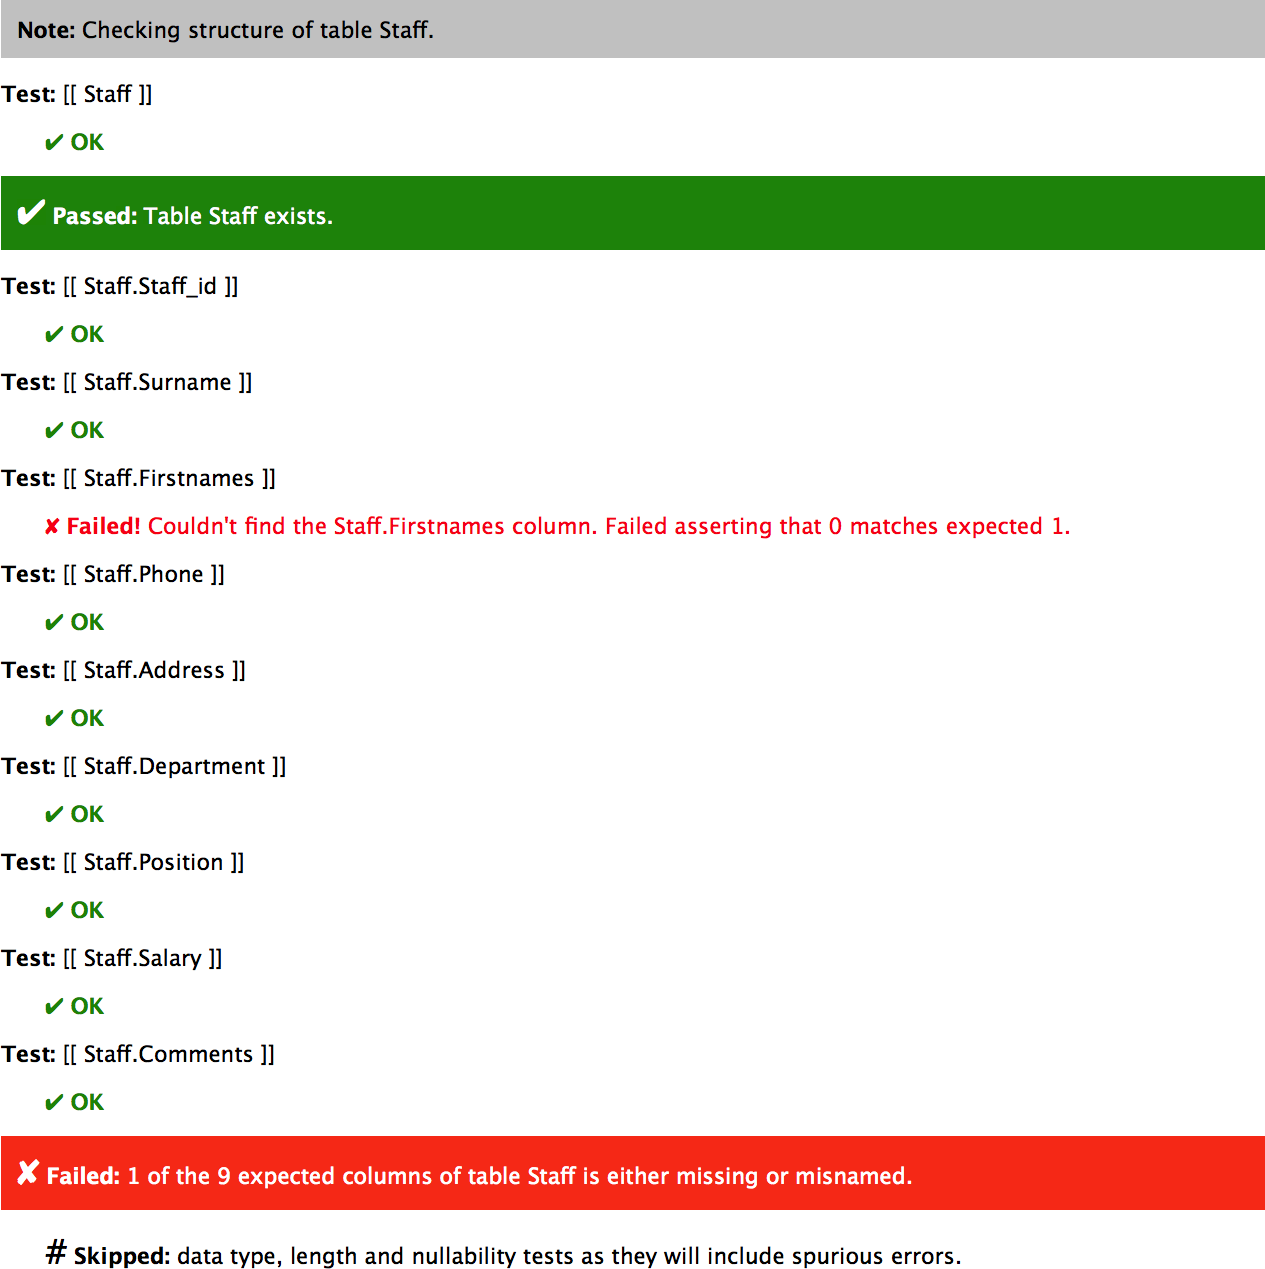
\includegraphics[width=0.95\columnwidth,keepaspectratio]{images/web_output.png}
    \caption{Example of student mode output (web app) for the \textsf{Staff} table.}
    \label{fig-student-output}
\end{figure}


The way that the system runs the tests is somewhat unusual, in two ways. First, database unit testing frameworks are generally designed around the concept of testing database-backed \emph{applications}, rather than testing the database itself. Second, in typical unit testing, the tests are essentially standalone code units that are automatically executed in an order determined by the unit testing framework. The framework resolves dependencies among tests and handles collation of test results internally, reporting only success, failure, or ``error'' back to the client. In fact, most unit testing frameworks appear to be designed to be called from a specific tool (e.g., the \texttt{phpunit} command line tool), rather than embedded as a library into other programs.

Our system effectively inverts (or perhaps subverts) this approach. The main driver explicitly creates test suites itself and executes them directly, listening for the results of each test and collating them. This is because we need to be able to control the order in which tests are executed. If the structural tests fail, there is little point in running the integrity tests, as they will only generate a stream of errors. Similarly, if a column is missing, there is no point in running the data type and length tests. (Note that while PHPUnit supports grouping of tests, dependencies can only be defined between individual tests, not between groups.)

It is quite feasible to add table properties and tests beyond those already mentioned, as the specification is encoded as ordinary PHP code and is therefore constrained only by what is possible in PHP. All a teacher needs to do is add custom properties to the table specification, then add tests that use those custom properties. Custom tests are easily registered with the appropriate test set (structure or integrity) using PHPUnit's \texttt{@group} annotation.

Students can check their schema (\textsf{Student's schema} in \cref{fig-architecture}) by loading it into their personal database account (i.e., creating the tables), then entering their database login credentials into a web application (\textsf{Web app} in \cref{fig-architecture}). This calls the main driver in student mode and accesses the student's schema directly using the provided credentials. Only the structural set of tests is run, and the output is displayed in the web browser. \Cref{fig-student-output} shows an example of the output produced by student mode for the \textsf{Staff} table in \cref{fig-ERD}.

A teacher can check further aspects of a student's schema using the \textsf{Console app} shown in \cref{fig-architecture}. To ensure a clean testing environment, the teacher does not connect directly to the student's database account, as the student may (for example) continue to use it for other coursework. Instead, the teacher loads the student's submitted schema code under a separate account used only for grading purposes, and erases the schema before moving to the next submission. The login credentials for the grading account are specified in the console application's configuration file.

Assuming that there are no syntax errors in the student's code,\footnote{If there are errors, then the student has clearly not met the minimum requirements!} the teacher then runs the console application, which calls the main driver in staff mode. The main driver connects to the pre-configured grading account, runs all the available tests, and displays the output in the terminal window. \Cref{fig-staff-output} shows an example of the output produced by staff mode for the \textsf{Product} table in \cref{fig-ERD}.


% ANSI terminal colours for Terminal.app; see https://en.wikipedia.org/wiki/ANSI_escape_code#Colors
% grey 203, 204, 205
% green 37 188 36
% red 194, 54, 33
\definecolor{test grey}{rgb}{0.796,0.800,0.804}
\definecolor{test green}{rgb}{0.145,0.737,0.141}
\definecolor{test red}{rgb}{0.761,0.212,0.129}

\tcbset{boxsep=0pt, boxrule=0pt, arc=0pt, left=0pt, right=0pt, top=0.5pt, bottom=0.5pt}

\newlength{\dothskip}
\setlength{\dothskip}{0.72cm}
\newlength{\dotvskip}
\setlength{\dotvskip}{-1.25ex}
\newlength{\codeskip}
\setlength{\codeskip}{-0.5ex}

\begin{figure}
    \ttfamily\scriptsize
    \begin{tabbing}
        0123\=\kill
        \tcbox[colback=test grey]{NOTE: Checking structure of table Product.} \\[\codeskip]
        TEST: [[ Product ]]  \\
        \>  \textcolor{test green}{+ OK} \\
        \tcbox[colback=test green]{+++ PASSED: Table Product exists.} \\[\codeskip]
        TEST: [[ Product.Product\_code ]]  \\
        \>  \textcolor{test green}{+ OK} \\[\dotvskip]
        \hspace*{\dothskip}\vdots \\
        \tcbox[colback=test green]{+++ PASSED: Table Product contains all the expected columns.} \\[\codeskip]
        TEST: [[ Product.Product\_code: data type is NUMBER | INTEGER ]]  \\
        \>  \textcolor{test green}{+ OK} \\[\dotvskip]
        \hspace*{\dothskip}\vdots \\
        \tcbox[colback=test green]{+++ PASSED: All columns of table Product have data types compatible with the}\\[\codeskip]
        \tcbox[colback=test green]{specification.} \\[\codeskip]
        TEST: [[ Product.Product\_code precision and scale = 8 (with scale 0) ]]  \\
        \>  \textcolor{test green}{+ OK} \\[\dotvskip]
        \hspace*{\dothskip}\vdots \\
        \tcbox[colback=test green]{+++ PASSED: All columns of table Product have lengths compatible with the} \\[\codeskip]
        \tcbox[colback=test green]{specification.} \\[\codeskip]
        TEST: [[ Product PK ]]  \\
        \>  \textcolor{test green}{+ OK} \\
        \tcbox[colback=test green]{+++ PASSED: Primary key of table Product exists.} \\[\codeskip]
        TEST: [[ Product PK: Product\_code ]]  \\
        \>  \textcolor{test green}{+ OK} \\
        \tcbox[colback=test green]{+++ PASSED: Primary key of table Product includes (only) the expected} \\[\codeskip]
        \tcbox[colback=test green]{columns.} \\[\dotvskip]
        \hspace*{\dothskip}\vdots \\
        \tcbox[colback=test grey]{NOTE: Testing constraints of table Product.} \\[\codeskip]
        TEST: [[ Product.Stock\_count accepts ``0'' ]]  \\
        \>  \textcolor{test green}{+ OK} \\
        TEST: [[ Product.Stock\_count accepts ``99999'' ]]  \\
        \>  \textcolor{test green}{+ OK} \\
        TEST: [[ Product.Restock\_level accepts ``0'' ]]  \\
        \>  \textcolor{test red}{- FAILED! Column Product.Restock\_level won't accept legal value 0.} \\
        \textcolor{test red}{Failed asserting that false is true.} \\
        TEST: [[ Product.Restock\_level accepts ``99999'' ]]  \\
        \>  \textcolor{test green}{+ OK} \\
        TEST: [[ Product.Minimum\_level accepts ``0'' ]]  \\
        \>  \textcolor{test red}{- FAILED! Column Product.Minimum\_level won't accept legal value 0.} \\
        \textcolor{test red}{Failed asserting that false is true.} \\
        TEST: [[ Product.Minimum\_level accepts ``653'' ]]  \\
        \>  \textcolor{test green}{+ OK} \\[\dotvskip]
        \hspace*{\dothskip}\vdots \\
        \tcbox[colback=test red, coltext=test grey]{--- FAILED: 2 of 8 legal values tested were rejected by a CHECK constraint.}
    \end{tabbing}
    \vskip-1ex
    \caption{Example of staff mode output (console app) for the \textsf{Product} table.}
    \label{fig-staff-output}
\end{figure}


\section{Evaluation}
\label{sec-evaluation}

Unfortunately, the system was conceived as a practical solution to a perceived teaching issue, rather than as a research project with formal evaluation in mind. We therefore did not carry out any user evaluations with students that used the system.

From the perspective of the teaching staff, we found that the total amount of time taken to grade the relevant assignment was reduced only a little, as the system only semi-automated the grading process, and we still needed to convert the system's output into corresponding grades and meaningful feedback (see \cref{sec-issues} for further discussion of this). There were also a surprising number of submissions that did not meet the minimum requirements and thus had to be manually graded. On a more positive note, the system did automatically ensure that all gradable elements were checked, which improved consistency, and made the subjective experience of grading much less painful.

However, we were able to analyze whether use of the system had any impact on student performance in the relevant assignment, as we had extensive historical data of student grades. We collated data for the period 2009--2016 (there are no data for 2017 because the course has been discontinued; see \cref{sec-issues}), which encompassed several different permutations of scenario and available system modes, as summarized in \cref{tab-data}. The assignment counted for 15\% of a student's total grade in 2009 and 2010, and 10\% in subsequent years. The grade distributions for the assignment in each year are shown in \cref{fig-distributions}.


\begin{table}
    \caption{Historical characteristics of the database implementation assignment, 2009--2016.}
    \label{tab-data}
    \begin{tabular}{rrrrll}
        \toprule
                &   Class   &   Median                          &   Mean                            &               &   Modes   \\
        Year    &   size    &   GPA\textsuperscript{\emph{a}}   &   (\%)\textsuperscript{\emph{b}}  &   Scenario    &   used    \\
        \midrule
        2009    &   46  &   --\textsuperscript{\emph{c}} &   77.5    &   ``postgrad''        &   --  \\
        2010    &   68  &   3.4 &   73.4    &   ``student records'' &   --  \\
        2011    &   64  &   3.9 &   71.8    &   ``used cars''       &   --  \\
        \midrule
        2012    &   75  &   3.4 &   69.2    &   ``BDL''             &   staff   \\
        2013    &   77  &   3.2 &   84.3    &   ``student records'' &   both \\
        \midrule
        2014    &   49  &   3.4 &   77.6    &   ``used cars''       &   both \\
        2015    &   71  &   3.0 &   69.2    &   ``used cars''       &   neither  \\
        2016    &   75  &   3.5 &   71.0    &   ``BDL''             &   staff   \\
        \bottomrule
        \multicolumn{6}{l}{\footnotesize \textsuperscript{\emph{a}} On a 9-point scale where C-- = 1, A+ = 9. Value is for the specified year only.}    \\
        \multicolumn{6}{l}{\footnotesize \textsuperscript{\emph{b}} For students who submitted the assignment.}    \\
        \multicolumn{6}{l}{\footnotesize \textsuperscript{\emph{c}} Complete GPA data for 2009 were not available.}    \\
    \end{tabular}
\end{table}


\begin{figure}
    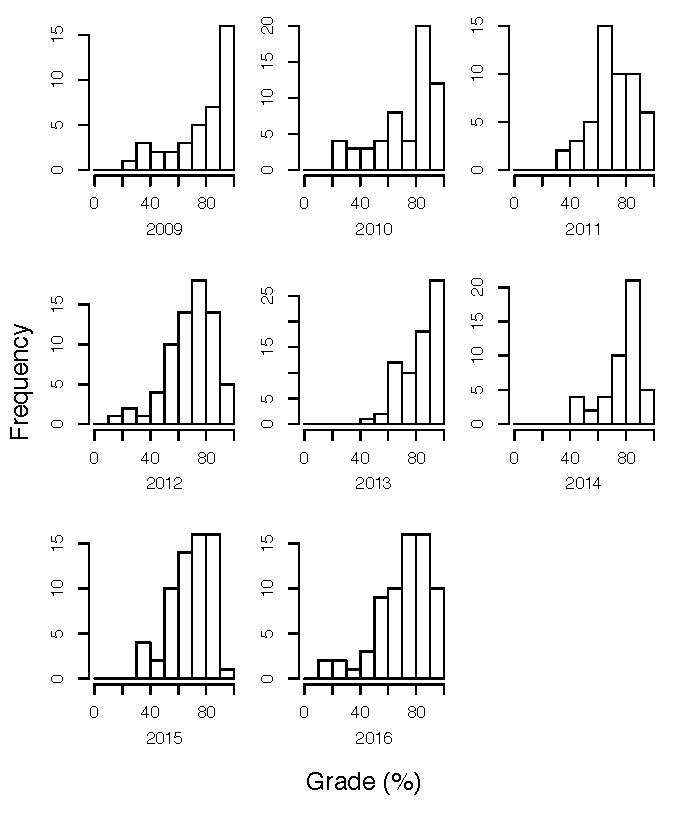
\includegraphics[width=\columnwidth,keepaspectratio]{grades_all_years.pdf}
    \caption{Comparison of grade distributions for the database implementation assignment, 2009--2016.}
    \label{fig-distributions}
\end{figure}


The horizontal rule in \cref{tab-data} between 2011 and 2012 marks a significant reorganization of the course's curriculum, and also a switch from first to second semester.\footnote{First semester at the University of Otago runs from March to June, second semester from July to October.} (2012 was also the year we deployed the first prototype of staff mode.) The horizontal rule between 2013 and 2014 marks a shift from second semester back to first semester. The system was not used at all in 2015 due to different staff teaching the course, and student mode was not made available in 2016 due to technical issues delaying its deployment beyond the point where it would be useful. These differences have provided us with a natural experiment with some interesting points for comparison.

The mean grade for the assignment drifted slowly downwards from 2009 to 2012. This reversed dramatically in 2013, however, the year we first deployed student mode. As can be seen in \cref{fig-distributions}, the grades are not normally distributed (they typically have negative skew), so we used a Mann-Whitney \emph{U} test to determine whether the increase in mean from 2012 to 2013 was statistically significant. This showed that the increase was highly significant (\(p \approx 10^{-9}\)). The 2013 mean was also significantly higher than both 2010 (\(p \approx 0.0002\)) and 2011 (\(p \approx 10^{-6}\)), but not significantly higher than 2009. The mean decreased significantly again in 2014 (\(p \approx 0.0012\)), the second year that the system was used, and even more dramatically in 2015 (\(p \approx 0.0005\)), when the system was not used at all. The increase from 2015 to 2016 was not significant.

Even more interesting, if we compare the performance between the years that student mode was not available (2009--2012 and 2015--2016, mean 71.6\%) and the years it was (2013--2014, mean 81.7\%), there is again a highly statistically significant increase in the mean (\(p \approx 10^{-8}\)). This difference is strikingly illustrated in \cref{fig-distribution-comparison}, which compares the grade distributions for both periods. During the period that student mode was available, the lowest grade awarded was 46\%, contrasted with a much longer tail of lower grades when student mode was not available. This strongly suggests that the introduction of student mode had a positive impact on students' ability to complete the assignment more effectively.


\begin{figure*}
    \centering
    \subfloat[]{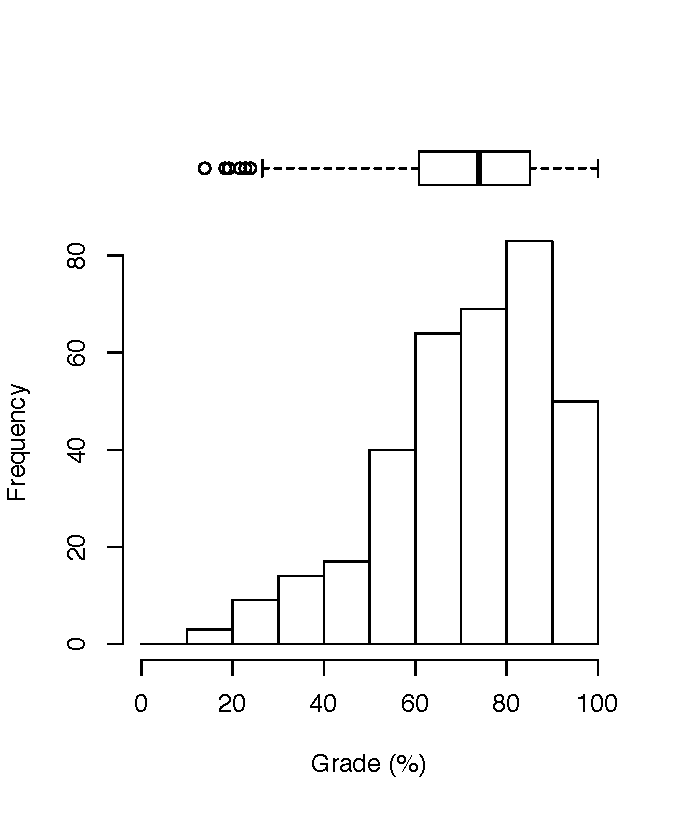
\includegraphics[trim=0 0 0 72,scale=0.6]{grades_without_student_mode.pdf}} \qquad
    \subfloat[]{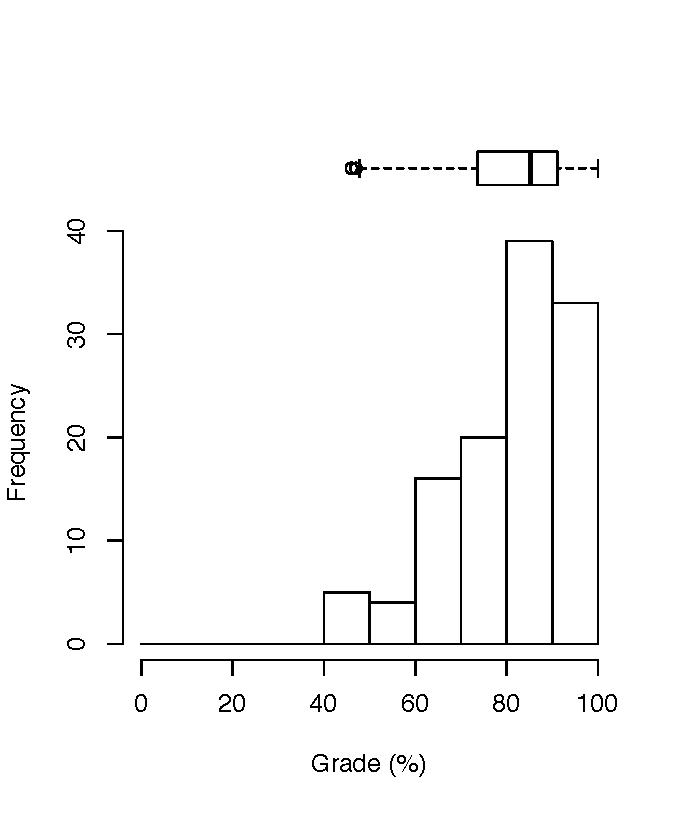
\includegraphics[trim=0 0 0 72,scale=0.6]{grades_with_student_mode.pdf}}
    \caption{Comparison of grade distributions (a) without student mode, (b) with student mode.}
    \label{fig-distribution-comparison}
\end{figure*}


There are some potential confounding factors to consider, however. First, not only was 2013 the first year that student mode was available, it was also the first year that the assignment specification was ``frozen'' (as discussed in \cref{sec-motivation}). It could be argued that this improved grades due to students having less flexibility, and thus less opportunity for misinterpretation, than in previous years. However, the assignment specification was also ``frozen'' in all subsequent years, and there is considerable variation in the grades achieved over this period, especially in 2015. It therefore seems unlikely that this was a factor in student performance.

Second, the observed effect may be due to the imposition of minimum requirements from 2013 onwards. Since any schema that met the minimum requirements would score at least 50\%, we could reasonably expect this to have a positive effect on the mean. If we compare with the period where minimum requirements were not enforced, we do find a significant increase in the mean, from 72.4\% to 75.6\% (\(p \approx 0.047\)). We argue, however, that this effect would be minimal in the absence of a convenient mechanism for students to check conformance with the minimum requirements. Indeed, for 2013--2014 when student mode was available, the mean (81.7\%) was significantly higher (\(p \approx 10^{-9}\)) than for 2015--2016 (70.2\%) when student mode was not available. This is further supported by no significant difference between the means for 2009--2012 and 2015--2016.

Third, the switch to second semester in 2012--2013 could have negatively impacted students' performance by increasing the length of time between their exposure to basic data management concepts in first year, and their entry into the second year database course. In effect, they had longer to forget relevant material they learned in first year. If so, we could reasonably expect the grades in second semester offerings of the course to be lower. However, mean grades for second semester offerings (76.9\%) were in fact significantly \emph{higher} (\(p \approx 0.015\)) than those for first semester offerings (72.9\%). This should not be surprising, given that 2013 (second semester) had the highest grades overall. This effectively rules out semester changes as a factor.

Fourth, perhaps the years with higher grades used less complex---and therefore easier---scenarios. To test this, we computed the following database complexity metrics for each of the four scenarios used: database complexity index (DCI) \cite{Sinha.B-2014a-Estimation}; referential degree (RD), depth of referential tree (DRT), and number of attributes (NA) \cite{Calero.C-2001a-Database,Piattini.M-2001a-Table}; database complexity (DC) \cite{Pavlic.M-2008a-Database}; and ``Software Metric Analyzer for Relational Database Systems'' (SMARtS)
\cite{Jamil.B-2010a-SMARtS}. The results are shown in \cref{tab-metrics}. All but the DRT metric clearly showed the ``BDL'', ``used cars'', and ``student records'' scenarios to be of comparable complexity, while the ``postgrad'' scenario was noticeably less complex. It therefore seems unlikely that scenario complexity is a factor in student performance. It is also interesting to note that the ``used cars'' scenario was used in both 2014 and 2015, and yet the 2015 grades were significantly \emph{lower} than those for 2014. The only clear difference here is that our system was not used in 2015.


\begin{table}
    \caption{Database complexity metrics for the scenarios used over the period 2009--2016.}
    \label{tab-metrics}
    \begin{tabular}{lrrrrrr}
        \toprule
            Scenario            &   DCI &   RD  &   NA  &   DRT &   DC  &   SMARtS  \\
            \midrule
            ``postgrad''        &   277 &   9   &   32  &   7   &   37  &   28.75   \\
            ``student records'' &   367 &   12  &   43  &   9   &   61  &   38.25   \\
            ``BDL''             &   370 &   11  &   50  &   8   &   59  &   40.75   \\
            ``used cars''       &   380 &   13  &   46  &   7   &   53  &   36.50    \\
        \bottomrule
    \end{tabular}
\end{table}


Fifth, class size could be a factor. We might plausibly expect a smaller class to have a more collegial atmosphere that promotes better learning. However, if we look at the sizes of the classes in \cref{tab-data}, we can see no discernible pattern between class size and performance. Indeed, both the best (2013) and worst (2012, 2015) performances came from classes of similar size (75, 77, and 71, respectively).

Sixth, it could be that better performance occurred in years where the students were just more capable in general. We obtained annual GPA data for the students enrolled in each year, and computed the median as an indication of the general capability of the class. Looking at \cref{tab-data}, we can immediately see that the year with the best results (2013) was also the year with the second-lowest median GPA (3.2). Contrast this with the poorer performance in 2012, where the median GPA was 3.4. In both years that student mode was available, median GPA was lower than or the same as in most other years, yet performance was better than in years with higher median GPA. This argues against the idea that we simply had a class full of very capable students in the better performing years.

Seventh, the timing of the assignment varied across the period, occurring either early (2012--2014), halfway (2009-2010), or late (2011, 2015--2016) in the semester, depending on the ordering of course content. The mean grade for early timing (77.0\%) was significantly higher than for both halfway (72.2\%, \(p \approx 0.019\)) and late (71.8\%, \(p \approx 0.013\)), while there was no significant difference between the halfway and late means. This suggests that scheduling the assignment early in the semester may have a positive effect on grades, and the period of early timing does overlap the period that student mode was available. However, as noted earlier there was a highly significant difference in mean between 2012 and 2013. There is also a smaller, but still significant difference in mean between 2012 and 2014 (\(p \approx 0.0015\)). We therefore conclude that while scheduling the assignment early in the semester may have had some positive effect on student performance, it does not explain all of the positive effect seen in 2013 and 2014.

Finally, perhaps the different weightings of the assignment (15\% in 2009--2010 vs.\ 10\% in 2011--2016) affected student motivation. It could be argued that the higher weighting in 2009--2010 provided a greater incentive for students to work more, as the potential reward was greater. If so, we should expect better performance in 2009--2010. Indeed, we do find this: the mean for 2009--2010 is 75.1\%, while that for 2011--2016 is 73.9\%, a statistically significant decrease (\(p \approx 0.034\)). However, since this change occurred well before our system was even conceived of, let alone implemented, it cannot be a factor in the improved performance seen in 2013 and 2014.

The sum of this evidence provides a strong argument in favor of student mode being the main factor in improving student grade performance in the database implementation assignment during 2013 and 2014. The most plausible explanation for this effect is that the direct feedback provided by the student mode web application enabled students to more effectively correct the structural aspects of their schema to meet the minimum requirements, giving them more time to work on the integrity aspects of their schema, and thus gain a higher grade.


\section{Known issues \& future work}
\label{sec-issues}

While the use of student mode in 2013 and 2014 appears to have had a beneficial effect on student performance in the database implementation assignment, there are some outstanding issues with the system that still need to be addressed.

Ideally, our system would automatically assign appropriate marks and generate meaningful feedback, and write both of these directly into a student management database. Currently, however, it only semi-automates the grading process, and it is still up to the teacher to interpret the test results, assign appropriate marks, and write feedback.

Automatically generating appropriate marks is not particularly difficult, and we have already implemented the core functionality required to assign mark penalties to different kinds of error. It would be a relatively simple extension to calculate marks based on these penalties and write them directly into a student management database.

Automatically generating meaningful feedback is problematic, however, due to the way that PHPUnit reports test failures. There is currently no way to control or suppress the messages generated by PHPUnit test assertions, most likely because PHPUnit is not designed to be used as an embedded library (as discussed in \cref{sec-design}). Individual tests can specify a meaningful message to be displayed, but PHPUnit will still generate somewhat obscure messages like ``Failed asserting that 0 matches expected 1'', which can be confusing for students.

One particularly tricky example we encountered was if a student failed to specify a precision for a numeric column, e.g., they declared a column as just \texttt{NUMERIC} rather than \texttt{NUMERIC(5)}. Most DBMSs will in this situation assign the maximum precision (e.g., 38 significant digits for Oracle). The student then sees a message ``Failed asserting that 38 matches expected 5'', and has no idea where the ``38'' came from.

This issue of unsuppressable assertion messages significantly constrained our ability to provide fully automatic, meaningful feedback to students. It may be that the only way to address this issue is to change the way PHPUnit works internally.

A second issue is that any schema that fails to meet the minimum requirements will result in a large number of errors due to missing tables.  This could be alleviated by more careful exception handling in the main driver.

Another issue is how students made use of the student mode web application. In 2013, students tended to misuse it as a ``schema compiler'': they would submit their schema, fix only the first issue reported (rather than attempting to fix as many as possible), immediately re-submit, and so on. We had not expected so high a request rate, so the system was only single-threaded and thus not designed to handle concurrent requests. Consequently the web application suffered from waits and timeouts. An initial workaround was to log all student access and warn those who were abusing the system. We later throttled the system by enforcing a short delay between attempts by the same student. Things improved in 2014 with careful management of student expectations, but longer term, the system should be redesigned to handle concurrent loads.

The system currently does not support behavioral aspects such as sequences, triggers, or stored procedures, as these are usually DBMS-specific in nature. It would not be difficult to add support for these, however, which could be included in the DBMS abstraction layer proposed in \cref{sec-design}.

Looking forward, it would be interesting to extend our system to help facilitate the teaching of SQL DDL, rather than just focusing on assignment grading. This has been done previously with several systems for SQL DML, as discussed in \cref{sec-literature} (e.g., \cite{Kenny.C-2005a-Automated,Kleiner.C-2013a-Automated,Mitrovic.A-1998a-Learning,Russell.G-2004a-Improving,Sadiq.S-2004a-SQLator}).

From 2017, we no longer have a dedicated second year database course. The main introduction to database concepts and SQL now occurs as part of our new (in 2017) first year ``Foundations of Information Systems'' course. This course attracted about 160 students in first semester, and about 100 students in second semester. Classes of this size further strengthen the argument for automated grading, and we are currently exploring whether our system could be used in this course in 2018. If this is feasible,  we intend to carry out user evaluations with the students.


\section{Conclusion}
\label{sec-conclusion}

In this paper we have described a novel system that semi-automates the process of grading SQL data definition code. To our knowledge, all prior work in this area has focused only on data manipulation statements such as \texttt{SELECT}, so extending this to data definition code is a key contribution of our system. The system also takes a novel approach to checking an SQL schema: rather than attempting to parse the SQL DDL code directly, it instead verifies that the schema conforms to a machine-readable version of the original specification. Finally, our system uses a unit testing approach to carry out the verification, which has not been used before in this context.

While no user evaluations of the system were carried out, analysis of student performance in a relevant database assessment shows a highly statistically significant increase in mean grade in the two years that the system was available for use by students. While we cannot be absolutely certain, analysis of all the factors involved strongly suggests that use of our system by students had a positive impact on their performance in this assessment. This is an encouraging result, which we will explore further in future work.


\bibliographystyle{ACM-Reference-Format}
\bibliography{Koli_2017_Stanger}

\end{document}
